\subsection{Slučaj upotrebe: Ažuriranje informacija o predstavi}

\subsubsection*{Kratak opis}

Reditelj ažurira informacije o predstavi i prosleđuje administratoru
radi unošenja tih podataka u sistem.

\subsubsection*{Akteri}
\begin{itemize}
    \item \textbf{Reditelj} -- pravi potrebne izmene za predstavu
    \item \textbf{Administrator} -- unosi izmene koje je dobio od reditelja u sistem
    \item \textbf{Sistem} -- izvršava se automatski
\end{itemize}

\subsubsection*{Preduslovi}
\begin{itemize}
    \item Predstava je već kreirana.
    \item Novi podaci su dostupni.
    \item Administrator je ulogovan u sistem i ima mogućnost da unese nove podatke.
\end{itemize}

\subsubsection*{Postuslovi}
\begin{itemize}
    \item Izmene su sačuvane.
\end{itemize}

\subsubsection*{Osnovni tok}
\begin{enumerate}
    \item Reditelj je odlučio da napravi neke izmene vezane za predstavu (npr. promena glumca, trajanja predstave, itd.).
    \item Dostavlja izmene administratoru.
    \item Administrator se loguje u sistem.
    \item Administrator nalazi predstavu i unosi nove podatke.
    \item Sistem proverava da li je validan unos novih podataka.
    \item Administrator dobija potvrdu da li su novi podaci validni.
    \item Administrator odlučuje da sačuva nove izmene.
    \item Sistem čuva nove izmene.
\end{enumerate}

\subsubsection*{Podtokovi: /}

\subsubsection*{Alternativni tokovi}

\paragraph*{A1: Izmene nisu validne}
\begin{itemize}
    \item Sistem obaveštava administratora da podaci nisu validni. Administrator obaveštava reditelja da podaci nisu validni i prekida sa unošenjem izmena. Slučaj upotrebe se završava.
\end{itemize}

\paragraph*{A2: Pogrešno uneti podaci}
\begin{itemize}
    \item Sistem obaveštava administratora da podaci nisu ispravni. Administrator proverava podatke i ispravlja ih. Slučaj se vraća na korak 5 osnovnog toka.
\end{itemize}

\subsubsection*{Specijalni zahtevi: /}

\subsubsection*{Dodatne informacije: /}

\begin{figure}[H]
	\centering
	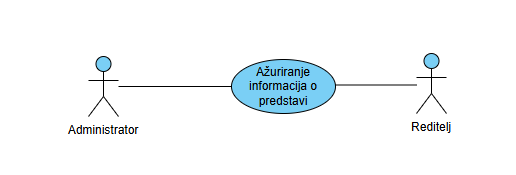
\includegraphics[width=\textwidth]{./Dijagrami/Dijagram slučajeva upotrebe/azuriranje_informacija_o_predstavi.png} 
	\caption{Dijagram slučaja upotrebe "Ažuriranje informacija o predstavi"}
\end{figure}

\newpage

